\documentclass[10pt,final,a4paper,oneside,onecolumn]{article}

%%==========================================================================
%% Packages
%%==========================================================================
\usepackage[a4paper,left=3.5cm,right=3.5cm,top=3cm,bottom=3cm]{geometry} %% change page layout; remove for IEEE paper format
\usepackage[T1]{fontenc}                        %% output font encoding for international characters (e.g., accented)
\usepackage[cmex10]{amsmath}                    %% math typesetting; consider using the [cmex10] option
\usepackage{amssymb}                            %% special (symbol) fonts for math typesetting
\usepackage{amsthm}                             %% theorem styles
\usepackage{dsfont}                             %% double stroke roman fonts: the real numbers R: $\mathds{R}$
\usepackage{mathrsfs}                           %% formal script fonts: the Laplace transform L: $\mathscr{L}$
\usepackage[pdftex]{graphicx}                   %% graphics control; use dvips for TeXify; use pdftex for PDFTeXify
\usepackage{array}                              %% array functionality (array, tabular)
\usepackage{upgreek}                            %% upright Greek letters; add the prefix 'up', e.g. \upphi
\usepackage{stfloats}                           %% improved handling of floats
\usepackage{multirow}                           %% cells spanning multiple rows in tables
%\usepackage{subfigure}                         %% subfigures and corresponding captions (for use with IEEEconf.cls)
\usepackage{subfig}                             %% subfigures (IEEEtran.cls: set caption=false)
\usepackage{fancyhdr}                           %% page headers and footers
\usepackage[official,left]{eurosym}             %% the euro symbol; command: \euro
\usepackage{appendix}                           %% appendix layout
\usepackage{xspace}                             %% add space after macro depending on context
\usepackage{verbatim}                           %% provides the comment environment
\usepackage[dutch,USenglish]{babel}             %% language support
\usepackage{wrapfig}                            %% wrapping text around figures
\usepackage{longtable}                          %% tables spanning multiple pages
\usepackage{pgfplots}                           %% support for TikZ figures (Matlab/Python)
\pgfplotsset{compat=1.14}						%% Run in backwards compatibility mode
\usepackage[breaklinks=true,hidelinks,          %% implement hyperlinks (dvips yields minor problems with breaklinks;
bookmarksnumbered=true]{hyperref}   %% IEEEtran: set bookmarks=false)
%\usepackage[hyphenbreaks]{breakurl}            %% allow line breaks in URLs (don't use with PDFTeX)
\usepackage[final]{pdfpages}                    %% Include other pdfs
\usepackage[capitalize]{cleveref}				%% Referensing to figures, equations, etc.
\usepackage{units}								%% Appropriate behavior of units
\usepackage[utf8]{inputenc}   				 	%% utf8 support (required for biblatex)
\usepackage{csquotes}							%% Quoted texts are typeset according to rules of main language
\usepackage[style=ieee,doi=false,isbn=false,url=false,date=year,minbibnames=15,maxbibnames=15,backend=biber]{biblatex}
%\renewcommand*{\bibfont}{\footnotesize}		%% Use this for papers
\setlength{\biblabelsep}{\labelsep}
\bibliography{../../bib}

%%==========================================================================
%% Define reference stuff
%%==========================================================================
\crefname{figure}{Figure}{Figures}
\crefname{equation}{}{}

%%==========================================================================
%% Define header/title stuff
%%==========================================================================
\newcommand{\progressreportnumber}{13}
\renewcommand{\author}{Erwin de Gelder}
\renewcommand{\date}{21 November 2018}
\renewcommand{\title}{Performance assessment of automated vehicles using real-world driving scenarios}

%%==========================================================================
%% Fancy headers and footers
%%==========================================================================
\pagestyle{fancy}                                       %% set page style
\fancyhf{}                                              %% clear all header & footer fields
\fancyhead[L]{Progress report \progressreportnumber}    %% define headers (LE: left field/even pages, etc.)
\fancyhead[R]{\author, \date}                           %% similar
\fancyfoot[C]{\thepage}                                 %% define footer

\begin{document}
	
\begin{center}
	\begin{tabular}{c}
		\title \\ \\
		\textbf{\huge Progress report \progressreportnumber} \\ \\
		\author \\ 
		\date
	\end{tabular}
\end{center}

\section{Previous meeting minutes}

\begin{itemize}
	\item We discussed the paper \emph{Have we collected enough field data?} with submission deadline of the 16th of November. I received feedback for everyone.
	
	\item Jan-Pieter asked whether I have a good idea on how to obtain the Graduate School Credits.
	
	\item We discussed the proposal for a student's graduation project. Bart mentioned that there is a poster session for MSc.\ students.
\end{itemize}

\section{Summary of work}

\begin{itemize}
	\item I submitted the paper \emph{Have we collected enough field data?} The notification of acceptance is before February 11. If the paper is accepted, it will be published in the Traffic Injury Prevention journal. If the paper is rejected, it will be published in the conference proceedings of the 26th International Technical Conference on Enhanced Safety of Vehicles (ESV). In any case, the final paper needs to be submitted no later than March 8.
	
	\item On the 25th of October, I spoke with Ludolf Meester from the Applied Probability department of the TU Delft about the work on aforementioned paper. The main conclusions of this discussion were:
	\begin{itemize}
		\item The method that is used is mathematically correct. 
		\item The biggest question is whether the Mean Integrated Squared Error (MISE) of the estimated probability density function (pdf) is the right measure for quantifying completeness.
		\item Especially for assessing the safety of automated vehicles, not the exact probability density is of concern, but whether certain parameters do occur or do not occur. Therefore, we might be more interested in the support of the underlying pdf instead of the MISE. The support can be thought of as the closure of the set of possible values of a the random variable.
		\item Ludolf Meester suggested to look into Extreme Value Theory (EVT). To illustrate the use of EVT: it is applied to define the requirements of the dikes of the Netherlands, as the dikes should be built such that a flood occurs only once in 10000 years \cite{dehaan1994extreme}.
	\end{itemize}
	
	\item It is a while ago since I showed something about the ``ontology''. I finally wrote down the results we have so far, see the attachment of this document. Some comments: 
	\begin{itemize}
		\item The whole ontology is represented by a domain model in Fig.\ 1 of the attachment. This domain model is a screen shot of Enterprise Architect. As I cannot edit the domain model (I can only see it), the naming of the classes and attributes is not always consistent. Please ignore the inconsistencies in the figure.
		\item Almost the whole ontology is also available at Python code.
		\item I do not expect major changes, but the ontology is not yet finished:
		\begin{itemize}
			\item It is not clear how (changing) conditions, such as weather and lighting, should be represented. 
			\item Scenarios that are found in the data can be described (we tried that). However, test cases, which are also scenarios and should therefore be described using the same ontology, are a bit different because the activities of the ego vehicle are not (necessarily) defined. Instead, the initial state and the objective (desired state) are defined. Currently, the initial state and the desired state are not described in this ontology.
			\item A scenario and a scenario class are currently connected through the method \texttt{falls\_into}. As it is not clear what this method actually does, it is not yet defined in Python.
		\end{itemize}
		\item Only the classes that are used to qualitatively describe a scenario are documented.
	\end{itemize}
	 
\end{itemize}

\section{Future plans}

\begin{itemize}
	\item I will start with a course on programming with R. This course is worth 5 GS credits.
	
	\item Finish the ontology and continue with the document describing the ontology.
	
	\item I already started working on a journal paper for the ontology. Given the new insights, I want to redefine the structure of this paper. For the next progress meeting, I want to have the draft structure of this paper ready.
	
	\item I mentioned in the Go/No Go report that I want to write a paper on our work in CETRAN. More specifically, I want to write a paper on so-called ``Milestone 3''.
	
	The goal of CETRAN is to define tests that evaluate the readiness of autonomous vehicles (AVs) to operate with ``high driving automation'' (level 4 according to J3016 by SAE \cite{sea2018j3016}). Therefore, CETRAN needs to develop three tests. The first test, i.e., ``Milestone 1'', evaluates the capability of the AV to be overtaken by a safety driver. Every AV that passes this test is allowed to perform test drives in a small region of Singapore (One-North). The second test, i.e., ``Milestone 2'', includes some basic tests that should demonstrate the capabilities of the AV to behave normally in rather common scenarios. Milestone 2 does not include critical test cases, i.e., test cases in which large accelerations are required to prevent an accident. Every AV that passes Milestone 2 is allowed perform test drives in a larger region of Singapore (mostly One-North and Buona Vista). CETRAN finished Milestone two months ago. In the coming months, CETRAN needs to develop Milestone 3. This milestone should be a \emph{methodology} to develop test cases (a methodology, because the test cases itself  depend on the vehicle under test and cannot be defined up front).
	
	One of the criticism of AV developers is that they need to pass milestone 2 (that is an agreement they have with the Singaporean government) right after the descriptions of the tests are distributed by CETRAN. This is impossible, according to the AV developers, because they need time to develop their vehicles to pass the tests. To prevent this situation for milestone 3, I think it would be good to publish the methodology that is used to define the tests some time \emph{before} the actual Milestone 3 is ready. 
	
	I want to take the lead for this paper. For the next progress meeting, I want to have a draft structure for this paper. This draft should also include the names of who can write what (other people from CETRAN need to contribute).
\end{itemize}


\printbibliography

\newpage
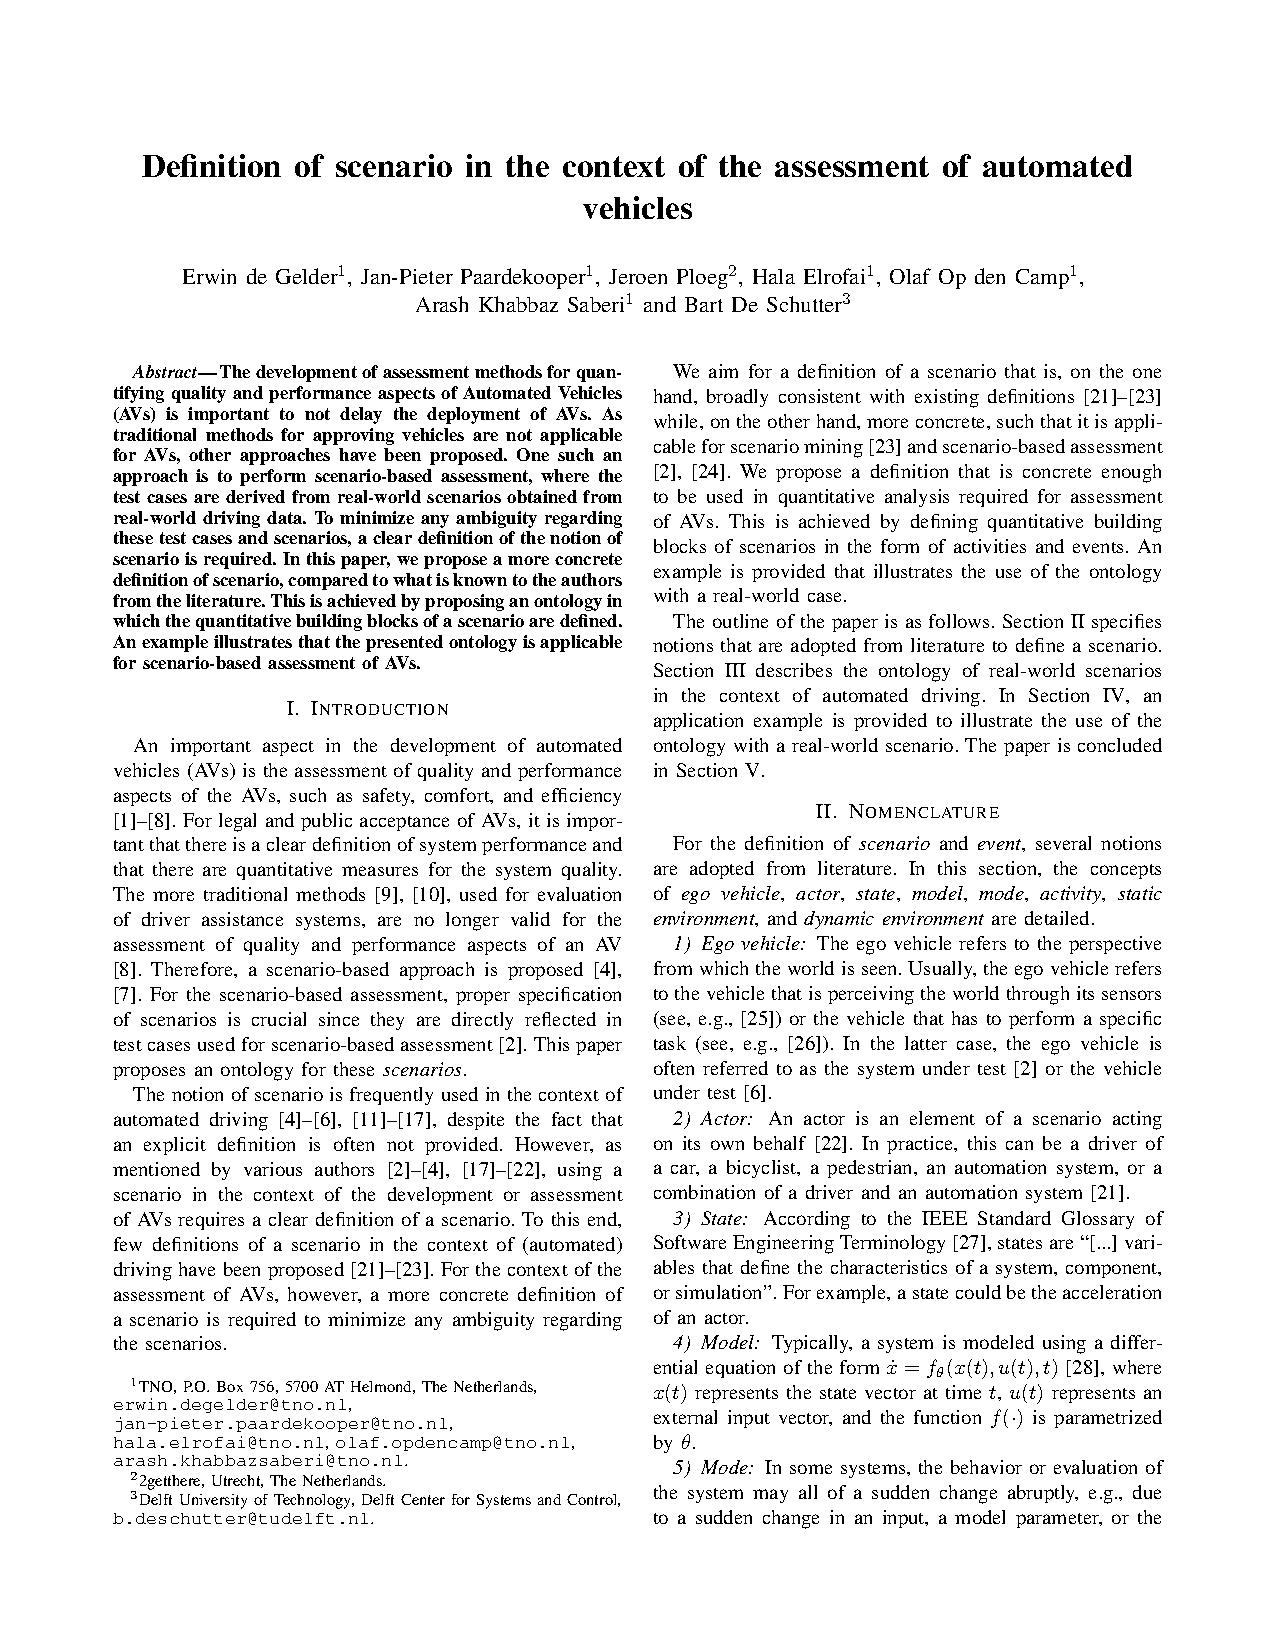
\includepdf[pages=-,pagecommand={},width=\paperwidth]{../../"20180710 Ontology"/ontology.pdf}

\end{document}